\documentclass[journal]{IEEEtran}
\usepackage{blindtext}
\usepackage{graphicx}
\usepackage{amsmath}
\usepackage{graphicx}%
\usepackage{url}%
\usepackage{abstract}%
\usepackage{csquotes}
\usepackage{amsthm}
\usepackage{amssymb}

\hyphenation{op-tical net-works semi-conduc-tor}

\usepackage[backend=biber]{biblatex}%
\bibliography{biblio}% The name of your .bib file


\begin{document}
%
% paper titlesdsd
% can use linebreaks \\ within to get better formatting as desired
\title{Damage localization based on vibrations}


\author{Benjamin Fasquelle, Nicolas Pompidor and Jimmy Rogala}

\newtheorem{remark}{Remark}

% The paper headers
%\markboth{Project}{}


% make the title area
\maketitle


\begin{abstract}
For aerospace, civil and mechanical engineering infrastructure, implementing a damage identification strategy is referred as a structural health monitoring.
With the help of accelerometers, a vibration analysis allows monitoring without the needs of human presence.
The damage identification can be divided into four levels: detection, localization, quantification and prediction.
We present existing methods for the detection and the localization of damage, and detail one of them, namely the Frequency Response Function interpolating method.
We analyse this method in a statistical sense and illustrate it with a simulation of a spring–mass system and a beam, and discuss the results.



\end{abstract}

\begin{IEEEkeywords}
Damage, Localization, Vibration, Health monitoring
\end{IEEEkeywords}


\IEEEpeerreviewmaketitle



\section{Introduction}


The process of implementing a damage identification strategy for aerospace,
 civil and mechanical engineering infrastructure is referred as a structural health monitoring (SHM) \cite{farrar2007introduction}.

In the most general terms, damage can be defined as changes in a system that negatively affect its current or future performance.
In general, a damage can be observed by comparing two different states of the system,
 one of which is supposed to represent the initial, and often undamaged, state.


It is of interest to detect damage in infrastructure as quickly as possible whether
 for the potential life-safety or economic impact.
Such detection requires industries to perform some form of SHM.

For instance, there are  no quantifiable methods to
 determine if buildings should be repaired after an earthquake yet.
SHM may one day provide the technology that can be used to significantly minimize
 the uncertainty associated with such post-earthquake damage assessments.
Thus additional catastrophes could be avoided.


Generally, the damage identification can be divided into four levels \cite{peeters2000system}:
\begin{itemize}
\item detection: Is the structure damaged or not?
\item localization: Where is the damaged area located?
\item quantification: What is the extent of damage?
\item prediction: What is the remaining service life of the structure?
\end{itemize}
\vspace{2mm}

Traditional methods of damage detection based on visual inspections or experimental techniques such as radiography
 or ultrasound allow to obtain detailed information about a local damage state but requires to know the area where it is located (and hope for easy access).
These techniques may be costly, taking a long time to be performed and impractical to detect damage in large urban areas.
 Furthermore, they may fail if damage is not visibly evident. This is why other global methods automated
 and based on sensor measurements were developed.



The purpose of this work is the analysis of a particular data-driven damage localization method,
 namely the FRF interpolation method \cite{dilena2015damage}. Our contribution is the development of a simulator to obtain acceleration measurement of different structures, a proposition of a variant of the FRF interpolation method, and a statistical analysis of the two methods.

This paper is organized as follows: In section II we  present the existing methods (model-based and data driven methods),
then in section III we present different models of vibrating structures required for what happens next. In section IV,  we talk about the localization using FRF interpolation method, in section V we detail our simulation used to obtain data and, finally, the experiences and its results in section VI.



\section{State of the art}

The use of methods based on recorded vibration responses proved to perform as valuable alternatives.
The general idea for vibration-based damage identification is that the damage affects the physical properties (mass, damping, and stiffness) of the structure, and this will cause detectable changes in modal properties (natural frequencies, modal damping, and mode shapes).
For instance, cracks cause reductions in stiffness. Therefore, by analyzing the dynamic properties of the structure a damage can be detected.
\\

Most of the different vibration based damage identification methods can be classified as data-driven or model-based.
% The model-based methods assume that a detailed numerical model of the structure is available for damage identification and, by vibration measurements, updates the model parameters.
% On another side, data-driven methods are based solely on the recorded response. These methods are interesting for a real-time damage identification but unavailability of a numerical model often hinders the estimation of damage severity.
 A third group includes data-driven methods that use finite element (FE) information without model updating.

\subsection{Finite Element model-based methods}

In model-based methods, damage is identified through the updating of a finite element (FE) model.
% Most of the time, modal characteristics is the experimental data used for damage assessment through FE model updating.% which are extracted from measured response time histories using modal analysis techniques.
Different types of modal data can be used. For changes in structural stiffness, model updating can be performed based only on modal parameters which are known to change with damage.
Note that model updating is often an ill-posed problem, requiring engineering expertise, that is difficult to automate.
 Detailed informations about model-based methods can be found in references
\cite{fritzen1998damage},
\cite{simoen2015dealing} and
\cite{teughels2005damage}.


\subsection{Data driven methods}

Data driven methods are inverse methods that use models based on response data recorded on the structure instead of physical models
\cite{limongelli2016towards}.
Here, a FE model isn't necessary, only recorded data are analyzed.
 In these methods, the damage parameter $D$ is the variation of a damage feature $d$ between the inspection $I$ and the reference $R$ configurations: %Damage-sensitive features are extracted from data and their changes used to identify damage in the structures so the damage parameter D in these method is the variation of the damage feature f between the inspection I and the reference R configurations.
% référence TOWARDS EXTRACTION OF VIBRATION-BASED DAMAGE INDICATORS
% nom pdf : fact sheet template_vibration based_final.pdf


\begin{equation}
D=d_{I} - d_{R}
\end{equation}

Data-driven methods do not require a FE model  and may be applied with a limited number of available signals (both responses and excitations).
To extract the damage features, different signal-processing tools can be used. Therefore, depending on the tool,  data-driven methods can be classified in Fourier-based methods, Time series method and Time-variant methods.
A more detailed description of these methods can be found in references %rajouter celles en-dessous
% Fassois S.D. and Sakellariou J.S. (2007) Time-series methods for fault detection and identification in vibrating structures. Phil. Trans. R. Soc. A. 365, 411–448. doi:10.1098/rsta.2006.1929.
\cite{fassois2007time} and
% Staszewski W. J.and Robertson A.N. (2007). Time–frequency and time–scale analyses for structural health monitoring. Phil. Trans. R. Soc. A. 365, 449–477. doi:10.1098/rsta.2006.1936.
\cite{staszewski2007time}.
The analyzed method in this paper belongs to this class.

\subsection{Combined data-driven and model-based methods}

A third group of methods for damage localization and quantification lies between the data-driven and model-based approaches.
Damage features are computed from both the data and the FE model, without updating the model.
% "This class is based on datadriven features from measurements of the reference and damaged states, which are confronted to a FE model of the structure to define damage indicators for the elements of the FE model,
% without updating its parameters" \cite{limongelli2016towards}. %rajouter référence au papier
% référence TOWARDS EXTRACTION OF VIBRATION-BASED DAMAGE INDICATORS
% nom pdf : fact sheet template_vibration based_final.pdf
% Maria Pina Limongelli, Eleni Chatzi, Michael D¨ohler, Geert Lombaert, Edwin Reynders
% https://hal.inria.fr/hal-01344178/document

\section{Vibration modeling}

In this section, we present the dynamic models for vibration analysis, and the Frequency Response Function (FRF) which is the base of the FRF interpolation method.

\subsection{Equation of motion}

The dynamic behaviour of a mechanical system consisting of $n$ degrees of freedom is described by following matrix differential equation:
\begin{equation}
M \ddot{q}(t) + C \dot{q}(t) + K q(t) = f(t)
\label{fondamental}
\end{equation}
where $q(t)$ is the displacement vector at a continous time $t$, $f(t)$ is the external force vector at $t$ and $M, C, K \in \mathbb{R}^{n \times n}$, are the mass, damping and stiffness matrices.

In real applications, only measurement data (forces $f$, most of accelerations $\ddot{q}$) are available, but matrices $M, C$ and $K$ are unknown.
For the purpose of simulating civil engineering structures, matrices $M, C$ and $K$ can be modeled through a
finite element approximation of the system with only $n$ dregrees of freedom.
The structure is divided in elements, and the global mass matrix $M$ and stiffness matrix $K$ are generated from the geometry and material
properties of the elements.

\subsection{Continous-time state-space model} %(model parameters and reduction):

For data analysis, Equation (\ref{fondamental}) is transformed. With the variable change $x =
\begin{pmatrix}
\dot{q} \\
q
\end{pmatrix}$, we obtain the state equation:
\begin{equation}
\dot{x}(t) = A_cx(t) + B_cf(t)
\end{equation}
 where
$A_c =
\begin{pmatrix}
0 & I \\
M^{-1}K & M^{-1}C
\end{pmatrix}$
and
$B_c=
\begin{pmatrix}
0 \\
M^{-1}
\end{pmatrix}$

In a practical vibration experiment, not all $n$ degrees of freedom of the structure are measured, but only
a subset. The observation equation is:
\begin{equation}
y(t) = C_cx(t) + D_cf(t)
\end{equation}

If it is assumed that all $n$ degrees of freedom are measured and that the sensors are accelerometers, we have
$C_c =
\begin{pmatrix}
M^{-1}K & M^{-1}C
\end{pmatrix}$
and
$D_c=
\begin{pmatrix}
M^{-1}
\end{pmatrix}$

Thus, the classical continuous-time state-space model is:
\begin{equation}
\left\{
\begin{array}{ll}
\dot{x}(t) = A_cx(t) + B_cf(t) \\
y(t) = C_cx(t) + D_cf(t)
\end{array}
\right.
\end{equation}

\subsection{Discrete-time state-space model} %(impulses response)

Up to now all equations were expressed in continuous time, whereas in reality
measurements are taken at discrete time instants.
So this model need to be converted to discrete time.
Another reason is that it is needed for performing simulations.

Thus, we choose a certain fixed sampling period $\Delta t$, and the continuous-time equations are discretized and solved at all
discrete time instants $k$ with $t = k \Delta t, k \in \mathbb{N}$.

The discrete-time state-space model is:
\begin{equation}
\left\{
\begin{array}{ll}
x_{k+1} & = A_dx_k + B_df_k \\
y_k & = C_dx_k + B_df_k
\end{array}
\right.
\label{discrete}
\end{equation}
where
\begin{equation}
\begin{array}{ll}
A_d = exp(A_c \Delta t) \\
B_d= (A_d - I) A^{-1}_c B_c \\
C_d = C_c \\
D_d = D_c
\end{array}
\end{equation}

\subsection{Frequency Response Function}

The FRF correspond to the transfer function of the system and reflects its dynamic behavior. In frequency domain, if $F(s)$ is the force that is applied on the system and $X(s)$ is the response of this force, the transfer function is given by:
\begin{equation}
H(s) = \frac{X(s)}{F(s)}
\end{equation}

We can express the theoretical transfer function with the matrices $M, C, K$. Indeed, in the frequency domain, we have
\begin{equation}
s^2 M X(s) + s C X(s) + K X(s) = F(s)
\end{equation}
Thus, the transfer function $H$ is:
\begin{equation}
H(s) = \frac{X(s)}{F(s)} = (s^2 M + s C + K)^{-1}
\label{changes}
\end{equation}

The FRF is evaluated at $s = i \omega$, with $\omega$ the pulsation.
In practice, we want to calculate the FRF of the system, for each sensor localization.
The FRF is calculated for each sensor location and each frequency $\omega_j = \frac{2\pi}{\Delta t} \frac{j}{N}$.
Here, we calculate an estimation of the FRF, called $H_1$ estimator \cite{cauberghe2004applied}. We suppose we have a vector of the forces $\{ f_k\}_{k=1}^N$ and a vector of the accelerations $\{ y_k\}_{k=1}^N$ for each sensor (the two vectors are size $N$). We need to be in frequency domain, so we calculate the discrete Fourier transform:
\begin{equation}
\begin{array}{ll}
F_j = \sum\limits_{k=1}^N f_k e^{-2i\pi kj/N} \ \ \ \ \ j \in \{1 ... N\} \\
Y_j = \sum\limits_{k=1}^N y_k e^{-2i\pi kj/N} \ \ \ \ \ j \in \{1 ... N\}
\end{array}
\end{equation}

Then we calculate the power spectra, i.e. the Auto Power spectra of the inputs and the outputs
and the Cross Power spectra between the inputs and outputs respectively given by:

\begin{equation}
\begin{array}{ll}
S_{ff}(j) = F_j F_j^H \ \ \ \ \ j \in \{1 ... N\} \\
S_{yf}(j) = Y_j F_j^H \ \ \ \ \ j \in \{1 ... N\}
\end{array}
\end{equation}
where $M^H$ is the Hermitian of the matrix $M$. Thus, the FRF is given by:
\begin{equation}
H_1(j) = S_{yf}(j) S_{ff}(j)^{-1}
\end{equation}

\begin{remark}
If we consider each sensor separately, $F_n$ and $Y_n$ are scalars, so we have:
\begin{equation}
\begin{array}{lll}
H_1(j) & = & S_{yf}(j) S_{ff}(j)^{-1} \\
& = & Y_j F_j^H (F_j F_j^H)^{-1} \\
& = & Y_j / F_j
\end{array}
\label{estimate}
\end{equation}
\end{remark}

\section{Localization using FRF interpolation method}

\subsection{The FRF interpolation method}

Changes due to damage induces changes in the FRF due to Equation(\ref{changes}). The FRF interpolation method analyses those changes based only on measurements of the system, computed from Equation(\ref{estimate}) without needing a FE model of the structure.

This method is presented in \cite{dilena2015damage}.
The main hypothesis underlying the method is that a concentrated damage reflects in a loss of spatial regularity of the
vibrational profile of a structure, compared with the reference (undamaged) state.

Figure \ref{theo} shows this loss of spatial regularity on the theoretical FRF, for a damage at the position 7.
We can see there is a loss of regularity at the position 7 for the damaged state. We can also see there is an iregularity at the position 2, but here the two states have the same iregularity, so it's not a loss of regularity compared to the reference state.

\begin{figure}[h!]
  \centering
  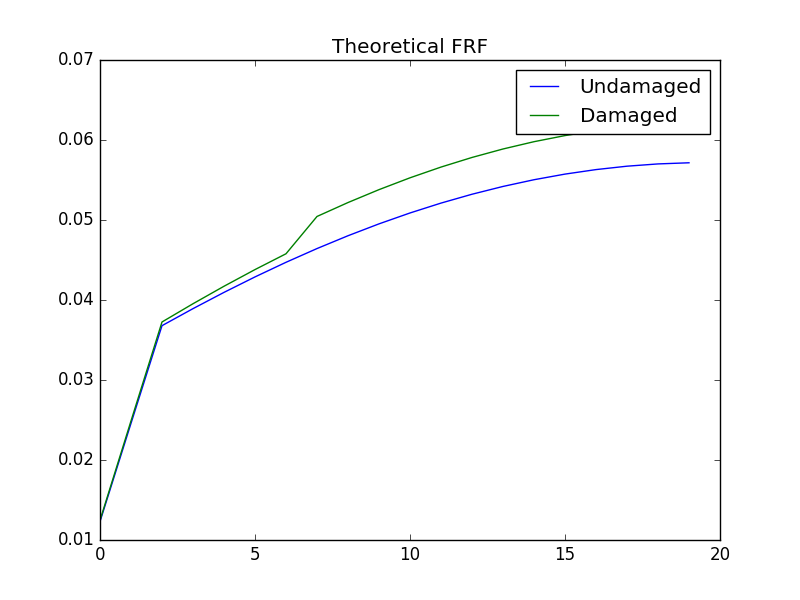
\includegraphics[width=0.3\textwidth]{images/theo60.png}
  \caption{Theoretical FRF for undamaged and damage states}
  \label{theo}
\end{figure}


We suppose that we have $n_s$ sensors, which are located along an axis $z$, and we denote them by
$\{z_l\}, l\in \{1 ... n_s\}$ (that is their position on the axis $z$). We also suppose we have $N$ measurements for each sensor.

For each sensor, we calculate the Frequency Response Function (FRF) from the acceleration's measures, at certain frequencies
(which are $\frac{k}{N}, k \in \{0 ... N-1\}$ with $N$ the size of the input and output vectors).

Thus, for each frequency and each sensor, we have the transfer function value. Let us denote $H_R(z_l,j) = H_1^l(j)$ ($l^{th}$ entry of $H_1$) the value of the transfer function for the sensor $z_l$ at the frequency line $j$, corresponding to $\omega_j$.

Then, we calculate for each sensor $z_l$ the cubic polynomial spline interpolation of the transfer functions $H_R(z_k,j)$ measured at all
the other instrumented locations $\{z_k\}, k\in \{1 ... n\}, k \neq l$: we denote it $H_S(z_l,j)$.
The cubic spline interpolation is a piecewise continuous curve, passing through each of the values.
There is a separate cubic polynomial interpolation for each interval, each with its own coefficients.
This is for this local aspect that we use this interpolation (other interpolations can also be used), since we want to detect local iregularities.
Cubic polynomial spline interpolations produce an interpolated function that is continuous through to the second derivative.

For these two transfer functions, we define the interpolation error $E(z_l,f_i)$ as the absolute value of the difference between recorded and interpolated FRFs:
\begin{equation}
E(z_l,j) = | H_R(z_l,j) - H_S(z_l,j) |
\end{equation}

We can see this error on the Figure \ref{interpolation_error}.


\begin{figure}[h!]
  \centering
  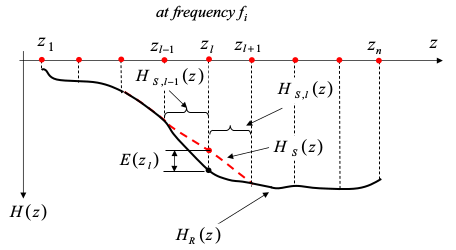
\includegraphics[width=0.4\textwidth]{images/interpolation.png}
  \caption{Interpolation error}
  \label{interpolation_error}
\end{figure}

Since we want to characterize each location $z_l$ with a scalar-valued error index, we introduce the norm of the error on the whole range of
frequencies:
\begin{equation}
E(z_l) = \sqrt{  \sum\limits_{j=1}^N  E^2(z_l,j) }
\label{error}
\end{equation}


Transfer function values obviously depend on the state of the structure. Hence, if the estimation of the error function
through Equation (\ref{error}) is repeated in the baseline (undamaged) and in the inspection (possibly damaged) configuration, then the
difference between the two values, denoted respectively by $E_0(z_l)$ and $E_d(z_l)$, can provide an indication about the existence of
degradation at location $z_l$:
\begin{equation}
\Delta E(z_l) = E_d(z_l) - E_0(z_l)
\end{equation}

An increase in the interpolation error between the reference configuration and the current configuration at a station $z_l$ , i.e.
$ \Delta E(z_l) > 0$, highlights a localized reduction of smoothness in the vibrational amplitude profile and, therefore, it is assumed
to be a symptom of a local variation of stiffness at $z_l$ associated with the occurrence of damage.


\subsection{Threshold}

The above analysis has been developed in a deterministic context. Several sources, such as temperature, nonlinear
behavior, soil structure interaction and noise in recorded data, can induce variations of the interpolation error even if no
damage occurs.

Thus, we can have different values of the error interpolation for a same state. The distributions of the erros for a state is close to a gaussian distribution. The problem is that the distributions for an undamaged and a damaged states can be near.

For a decision that an interpolation error belongs to the healthy or damaged state, once have to determine a threshold $E_T$, such as $ \Delta E(z_l)$ must be taller than $E_T$ to have a high probability of identification of a damage at location $z_l$. Indeed, as we can see in the Figure \ref{proba}, the curves which represent the fact to have a damage or not have a share area: if the interpolation error $ \Delta E(z_l)$ is in this area, one can commit two errors:
\begin{itemize}
\item if it is in the red area (FP), once can detect a damage since there isn't one (false alarm).
\item if it is in the green area (FN), once can not detect a damage since there is one (missing alarm).
\end{itemize}


\begin{figure}[h!]
  \centering
  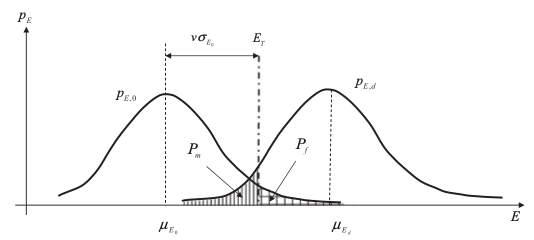
\includegraphics[width=0.4\textwidth]{images/gaussiennes.png}
  \caption{Probabilities of false and missing alarm}
  \label{proba}
\end{figure}

\begin{figure}[h!]
\begin{center}
\begin{tabular}{|c|c|c|}
\hline
\ & Damaged & Undamaged \\ \hline
Detected & TP & FP \\ \hline
No detected & FN & TN \\ \hline
\end{tabular}
\end{center}
\caption{True/False positives and negatives}
\label{TFPN}
\end{figure}

Now, to denote corect detection (or no detection), we will use the terms true positives and negatives, to denote missing alarms we will use false negatives and for false alarms, we will use false positives.

In our experiences, we measure the number of true/false positives and negatives. The Figure \ref{TFPN} present the notations used for the number of true/false positives and negatives.

To evaluate the two methods, we use the specificity predictive factors, which are
$\frac{TP}{TP + FP}$ and $\frac{TN}{TN + FN}$. The first correspond to the probability that there is a damage when we detect one, and the second correspond to the probability there isn't any damage when we detect nothing. A good method has the two factors near to 1.


\subsection{A variant of the method}

We propose here a variant of the FRF interpolation method. While we have worked on the implementation of the original method, we have observed the theoretical FRF to see if the FRF interpolation method worked on that. We noticed that the following procedure may magnify irregularities of the FRF:
\begin{itemize}
\item first, compute the difference between the FRF
\item second, compute the interpolation error on this difference
\end{itemize}

Figure \ref{theodiff} shows the difference betweem the two FRF, and we can see the loss of spatial regularity (damage at position 7).
In comparison with the Figure \ref{theo}, we can see here there is only one iregularity: the fact to compute the difference before the interpolation erase iregularity when they are in the two states. With the initial method, they are also erase when we compute the difference between the interpolation errors.

\begin{figure}[h!]
  \centering
  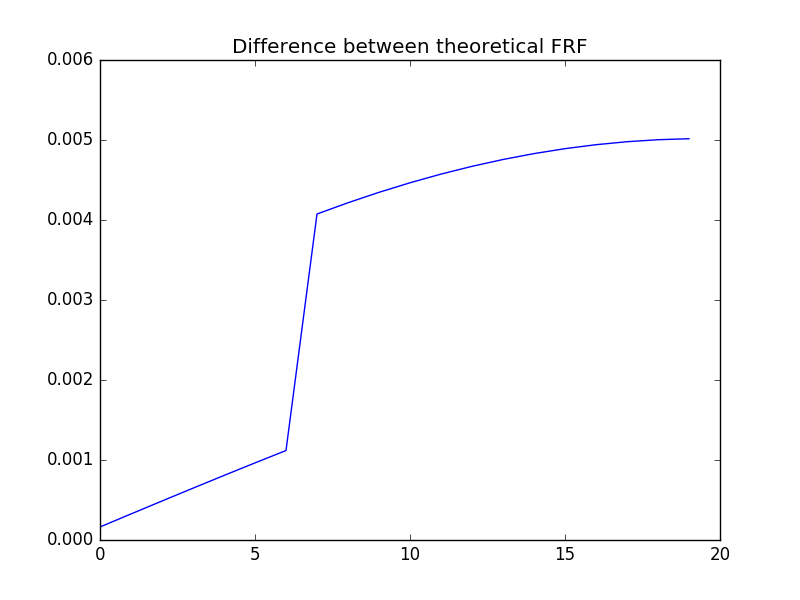
\includegraphics[width=0.3\textwidth]{images/theodiff60.png}
  \caption{Difference betweem theoretical FRF of undamaged and damage states}
  \label{theodiff}
\end{figure}


Thus, we also study in this paper a variant of the FRF interpolation method . The only difference with the original method is the order of the steps:
\begin{itemize}
\item Compute the FRF
\item Compute the difference between the FRF of reference and the FRF of the studied state, for each frequency
\item Compute the interpolation error of these differencies
\item Compute the sum of the interpolation errors at each frequency
\end{itemize}

From now on, to tell the difference between the two methods, we shall call our variant the FRF difference method.



\section{Simulation}


We have implemented a simulation to obtain the data used to analyse the methods of localization. To explain it, we detail here the following system we used for our experiments: $n$ masses, connected
through springs and dampers. We denote the masses $\{m_i\}_{i=1}^n$, the springs stiffness $\{k_i\}_{i=1}^n$ and the dampers $\{c_i\}_{i=1}^n$ (see Figure \ref{springs}).

\begin{figure}[h!]
  \centering
  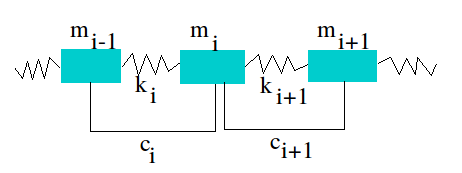
\includegraphics[width=0.4\textwidth]{images/ressorts.png}
  \caption{Masses connected through springs and dampers}
  \label{springs}
\end{figure}

For the simulation, we use the discrete-time state-space model (Equation (\ref{discrete})). First, we establish the matrices $M, C, K$. In this case, the matrices $M$ and $K$ are given by:
\begin{equation}
\begin{array}{l}
M =
\begin{pmatrix}
m_1\\
&\ddots\\
&&m_n
\end{pmatrix}
\\
K =
\begin{pmatrix}
k_1 + k_2 & - k_1 \\
- k_1 &\ddots\\
& -k_i & k_i + k_{i+1} & -k_{i+1} \\
&&&\ddots& -k_n\\
&&& -k_n & k_n
\end{pmatrix}
\end{array}
\end{equation}


Due to the lack of identifiable or measurable material
constants that govern the global damping behaviour of a structure, it is generally
impossible to assemble the damping matrix C in the same way as M and K.
Thus,we consider Rayleigh damping, i.e. a linear combination of the mass and stiffness matrix:
\begin{equation}
C = \alpha M + \beta K,\ \ \ \ \ \alpha, \beta \in \mathbb{R}_+
\end{equation}

With these matrices, we can calculate the matrices $A_c, B_c, C_c$ and $D_c$. To calculate the matrices $A_d, B_d$, we have to define the
sampling period $\Delta t$. We need the frequencies of the system, because we have to respect the Nyquist–Shannon sampling theorem.
To determine the Nyquist frequency which needs to be larger than the frequencies of the system, we calculate the eigenvalues of $A_c$. Indeed, we have the link between the eigenvalues $\{\lambda_j\}_{j=1}^n$ and the frequencies of the system $\{f_j\}_{j=1}^n$:
\begin{equation}
\lambda_j = - \omega_j \xi_j \pm i \omega_j \sqrt{1 - \xi_j^2}
\end{equation}
where $\omega_j = 2 \pi f_j$ and $\xi_j$ is the damping ratio.

\begin{remark}
We can see that:\\
$|\lambda_j| = \sqrt{\omega_j^2 \xi_j^2 + \omega_j^2 (1 - \xi_j^2)} = \omega_j$
\end{remark}

\begin{remark}
The matrix $A_c$ has $2 \times n$ eigenvalues, but we obtain $n$ frequencies (for each eigenvalues, another one is its conjugated complex).
\end{remark}

Now, we have the sampling period:
\begin{equation}
\Delta t = 2 \times max_{j \in \{1 ... n\} } f_j
\end{equation}

So we can calculate the matrices $A_d, B_d$ and make the simulation with the discrete-time state-space model (Equation (\ref{discrete})). To simulate the forces $f_k$, we use a white noise.


We can also use our simulation with other structures, like a beam, if we know the matrices $M$, $K$, $C$ and the impact of a damage on these matrices.
We will also validate the FRF interpolation method with a beam in this paper, but we don't detail the matrices $M$, $K$, $C$.


\section{Analysis}

For the following simulation results, we consider a system with 20 masses. We put a sensor on each mass. For the damaged state, we lower the stiffness of the spring between sensors 6 and 7. The values of the FRF on the figures are the norm of the complex FRF values.


\subsection{Data presentation}

Figure \ref{frf_freq} presents results of the FRF on the simulation data: here is the curve of the FRF of one sensor, against frequencies. We can see peaks which are at the natural frequencies of the system.


\begin{figure}[h!]
  \centering
  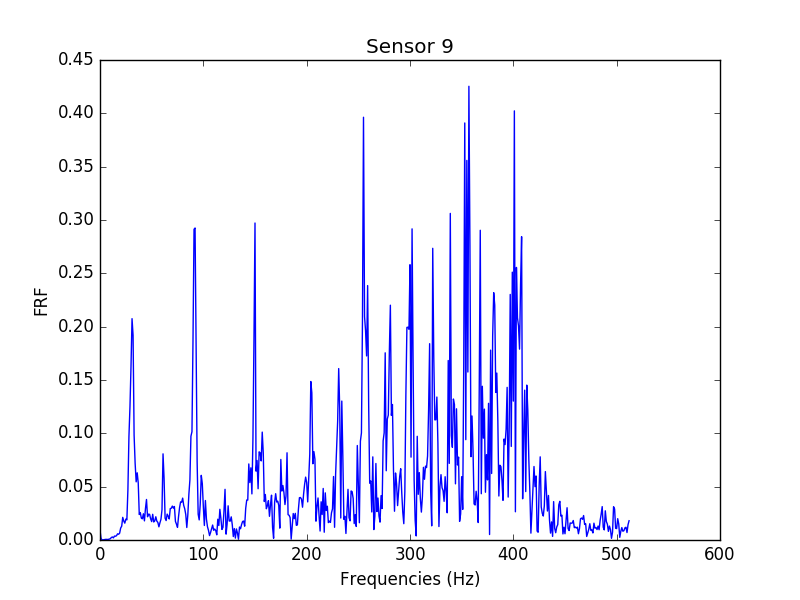
\includegraphics[width=0.3\textwidth]{images/frf_one_sensor.png}
  \caption{FRF of one sensor against frequencies}
  \label{frf_freq}
\end{figure}

Figure \ref{frf_sensors} presents results of the FRF for all the sensors at one frenquency. Curves aren't as regular as the theoretical FRF, but we can see clearly the iregularity between sensors 6 and 7 (there is 10\% of damage here).


\begin{figure}[h!]
  \centering
  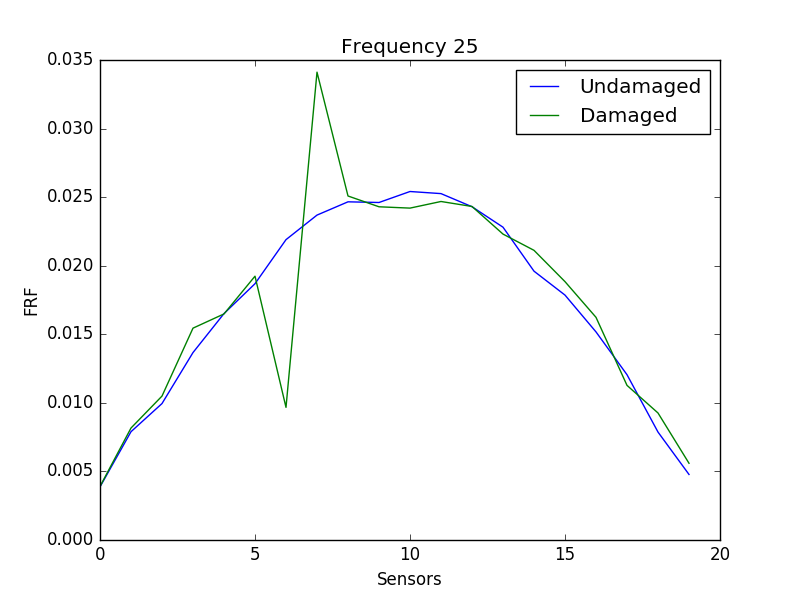
\includegraphics[width=0.3\textwidth]{images/frf_one_frequency.png}
  \caption{FRF for one frequency against sensors}
  \label{frf_sensors}
\end{figure}


\subsection{FRF interpolation method results}

To test the localization, we compute a threshold for each sensor. Then, an interpolation error above this threshold indicates damage. With the FRF interpolation method, we have computed two thresholds from 100 experiments with the undamaged state. The first is the error just below the maximum of the 100 errors computed. The second is computed from the statistics of the 100 errors computed: we suppose that the error follows a normal distribution, and we choose the threshold at 95\% of this distribution.

From now on, the majority of the figures will show four curves:
\begin{itemize}
\item in dark blue: results of the FRF interpolation method with a threshold at 99\% of the reference errors
\item in green: results of the FRF interpolation method with a threshold at 95\% of the reference distribution
\item in red: results of the FRF difference method with a threshold at 99\% of the reference errors
\item in blue : results of the FRF difference method with a threshold at 95\% of the reference distribution
\end{itemize}

To distinguish the two methods with the two thresholds, we denote them with the color initials: the first one DB, the second one G, the third one R and the last one B.

\subsubsection{Without noise}

Figure \ref{damage30} presents the results of the localization of a damage of 30\% between sensors 6 and 7, without noise.
It shows the percent of detection of a damage against its position.
We can see that the damage between sensors 6 and 7 are always detected, but there is also detection on other sensors (that is false positives).

\begin{figure}[h!]
  \centering
  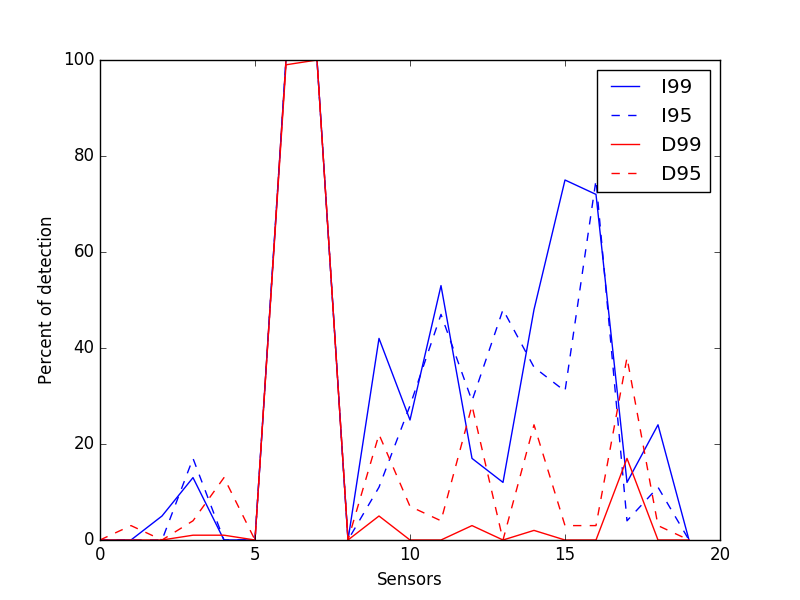
\includegraphics[width=0.4\textwidth]{images/damage30percent.png}
  \caption{Damage detection rate for a damage between sensors 6 and 7 (without noise)}
  \label{damage30}
\end{figure}



Figure \ref{detect} presents the percent of detection of a damage between sensors 6 and 7 against the damage extent (a single damage is always simulated on sensor 7). We can see here that below 5\% of damage, none of the methods detect the damage more than 50\% of the time, but we can see that B is the best: at 10\% of damage, it reach 90\% of detection, while the others are below 30\%. However, at 15\% of damage, it's DB and G which are the best, with 100\% of detection. B reaches 100\% of detection at 20\% of damage, and R reaches it at 30\% of damage. Here, R seems to be the worst.

\begin{figure}[h!]
  \centering
  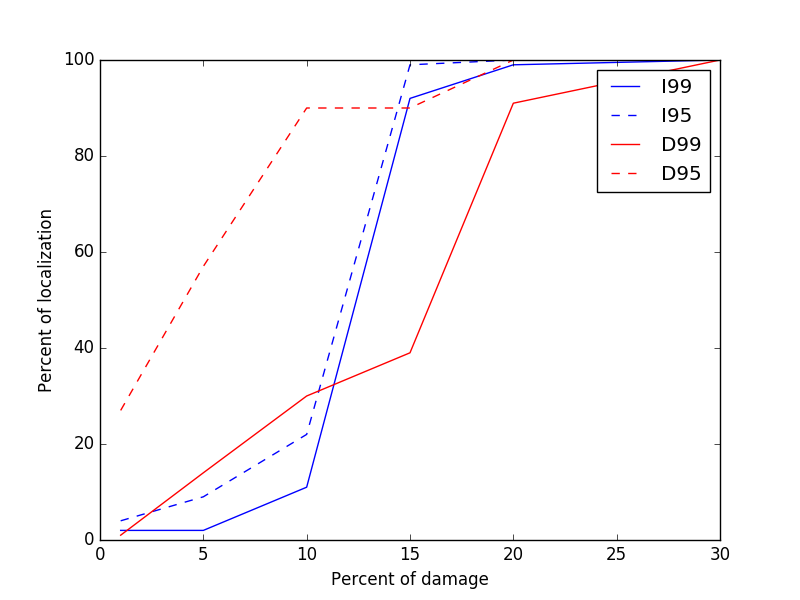
\includegraphics[width=0.4\textwidth]{images/detect.png}
  \caption{Damage detection rate against damage (without noise)}
  \label{detect}
\end{figure}


Figure \ref{fp} presents the percent of false positives against the damage percent. Here, R is the best: around 2\% of false positives regardless of the percent of damage, while the others are between 5\% and 25\%.


\begin{figure}[h!]
  \centering
  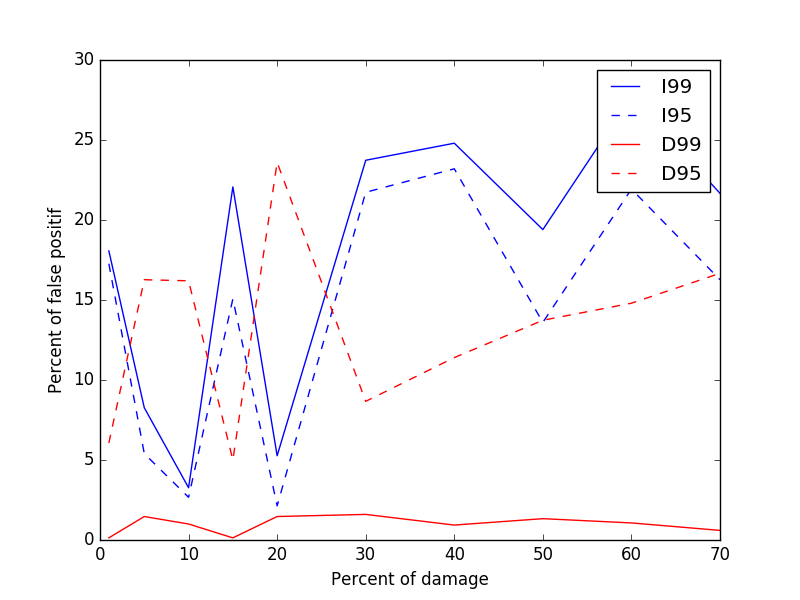
\includegraphics[width=0.4\textwidth]{images/fp.png}
  \caption{False positives rate against damage (without noise)}
  \label{fp}
\end{figure}



\subsubsection{With noise}



Figure \ref{damage30noise} presents the results of the localization of a damage of 30\% between sensors 6 and 7, where noise (5\%) has been add at the measurement. We can see that results are similar that without noise.


\begin{figure}[h!]
  \centering
  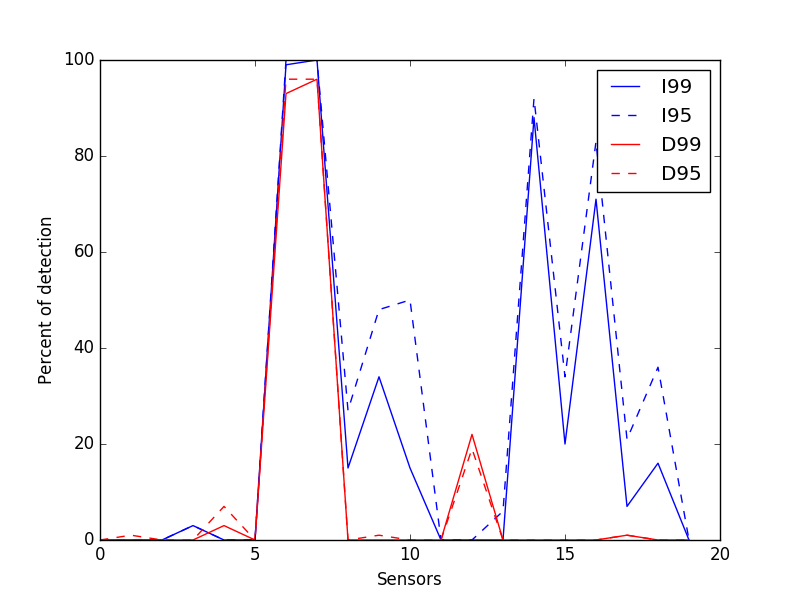
\includegraphics[width=0.4\textwidth]{images/damage30percent004noise.png}
  \caption{Damage detection rate for a damage between sensors 6 and 7 (with 5\% of noise)}
  \label{damage30noise}
\end{figure}

However, we can see on Figure \ref{detect_noise} that the rate of true positives is impacted by the noise: the G and BD methods reach 100\% of detection at 20\% of damage and the R and BL methods reach it at 40\% of damage.


\begin{figure}[h!]
  \centering
  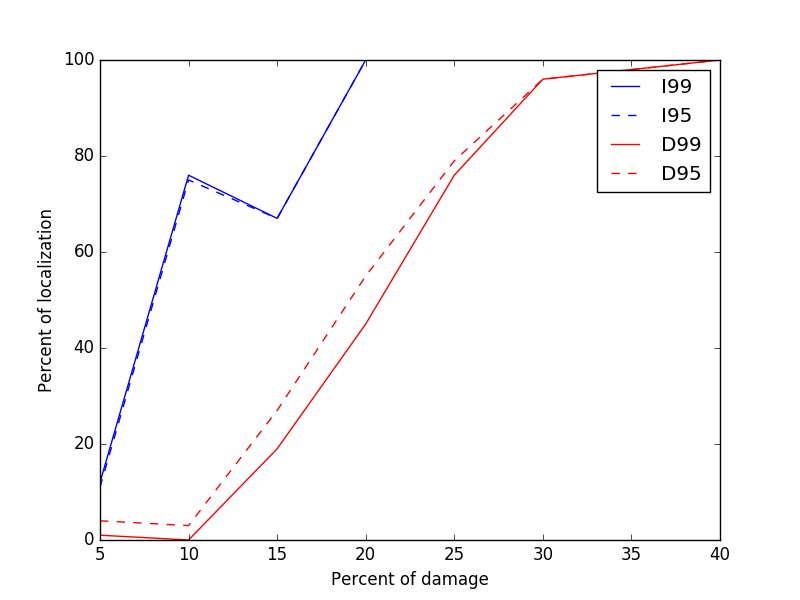
\includegraphics[width=0.4\textwidth]{images/detect_noise004.png}
  \caption{Damage detection rate against damage (with 5\% of noise)}
  \label{detect_noise}
\end{figure}

For the false positives rate, we can notice that the R method is always the best, but the BL method is better than without noise.


\begin{figure}[h!]
  \centering
  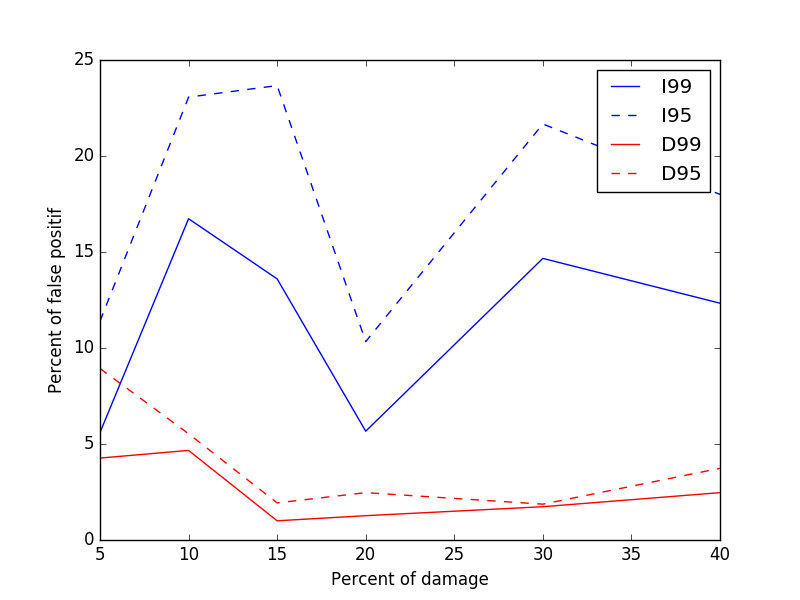
\includegraphics[width=0.4\textwidth]{images/fp004.png}
  \caption{False positives rate with 5\% of noise}
  \label{fp_noise}
\end{figure}


With the noise, we can so do two observations: first, the FRF interpolation method has a better localization for small damages than the FRF difference method, second,  the FRF difference method has a better false positives rate than the FRF interpolation method.


\subsection{Eliminate the false positives to improve the efficiency}

First, we present here the the predictive factors for our methods.

Figure \ref{pred} shows the predictive positive and negative factors. For the positive one, we can see that the R method is the best. For the negative one, we can see that all the method reach 1 at 30\% of damage, and are a factor higher than 0.9 for small damages.

\begin{figure}[h!]
  \centering
  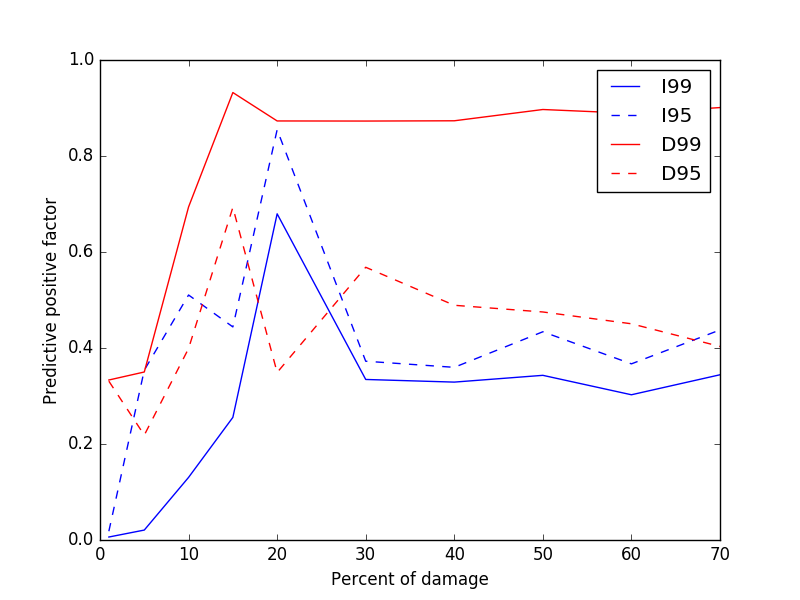
\includegraphics[width=0.4\textwidth]{images/pred.png}
  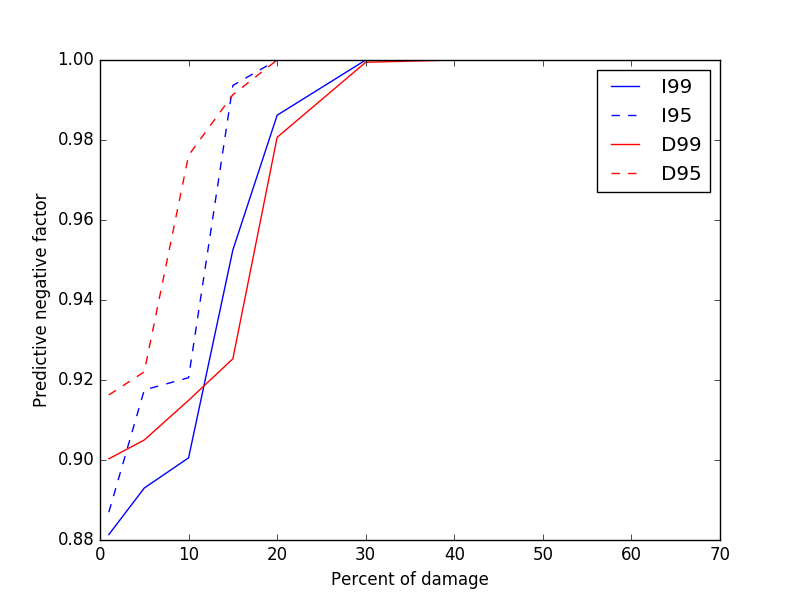
\includegraphics[width=0.4\textwidth]{images/pred_neg.png}
  \caption{Predictive positive and negative factors}
  \label{pred}
\end{figure}

%Figure \ref{pred_neg} shows the predictive negative factor with this method. 
%\begin{figure}[h!]
%  \centering
%  \caption{Predictive negative factor}
%  \label{pred_neg}
%\end{figure}

We can see that the predictive negative factor isn't bad, but the positive one can be better. To improve it, we must have less false positives. We try to remove them with the next idea: the difference between the threshold and the computed values is larger on the damage than on other sensors. As the damage is localized on one spring, so between two sensors, we apply the next algorithm to determine where is the damage:
\begin{itemize}
\item We compute the error values
\item We make the difference with the threshold
\item We keep only the two highest values, and we detect a damage only if they are positives
\end{itemize}

\begin{figure}[h!]
  \centering
  \includegraphics[width=0.4\textwidth]{images/detect_max_10percent.png}
  \caption{}
  \label{detect_max}
\end{figure}

Figure \ref{detect_max} shows the results of this method. We can see that all the false positives are eliminated.


\begin{figure}[h!]
  \centering
  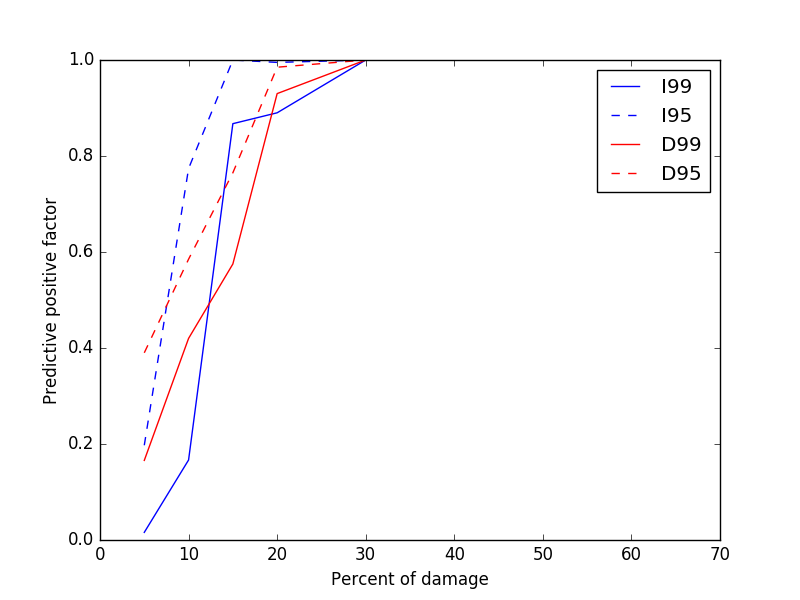
\includegraphics[width=0.4\textwidth]{images/pred_max.png}
  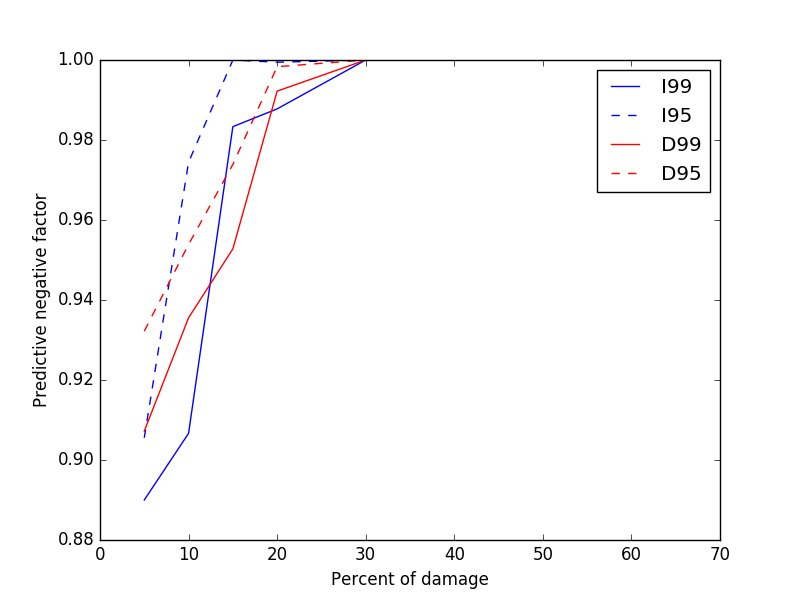
\includegraphics[width=0.4\textwidth]{images/pred_neg_max.png}
  \caption{Predictive positive and negative factors with elimination of false positives}
  \label{pred_max}
\end{figure}

Figure \ref{pred_max} shows the predictive factors with this method. For the positive one, we can see that all the method reach 1 at 30\% of damage. That is what you wanted to obtain with the elimination of the false positives. For the negative one, we can see that this factor is similar at the factor for the initial methods.

We have here improved the methods, because we eliminate the false positives. The only requirement is to have a detection method. We can notice that all the methods are perfect with damage extent higher than 30\%: in this case, the methods always have a correct localization.

\subsection{FRF interpolation method on a beam}

We test our localization on another structure: a beam. We don't detail this model in this paper, we just use it to verify our methods. The damage is localized between the sensors 4 and 5.

Figure \ref{beam_curve} shows two FRF, one for the undamaged state and the second for the damaged one, at a fixed frequency. We can easily see there is an irregularity at the sensor 4.

\begin{figure}[h!]
  \centering
  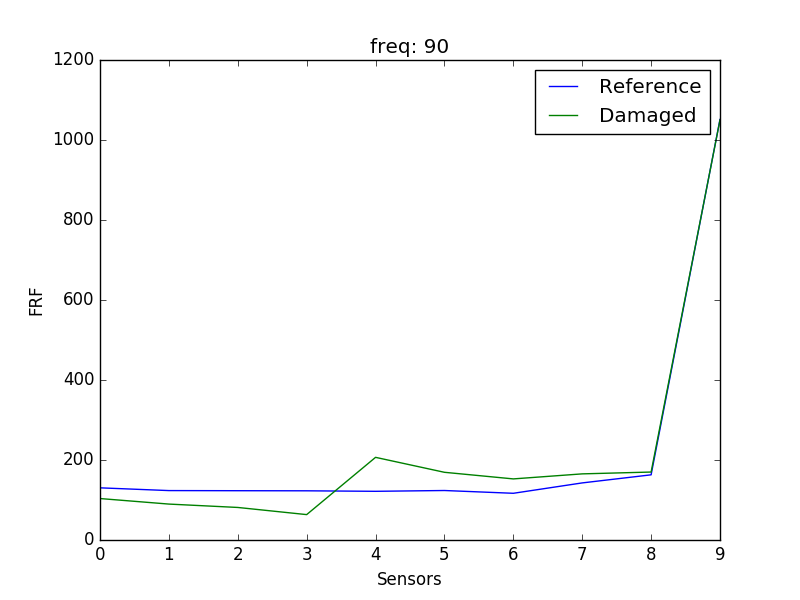
\includegraphics[width=0.4\textwidth]{images/poutre_curve2.png}
  \caption{}
  \label{beam_curve}
\end{figure}


Figure \ref{beam_error} shows the computed error. We can see that there are only two sensors with a positiv error, which are the sensors 4 and 5. Thus, the localization is good.

\begin{figure}[h!]
  \centering
  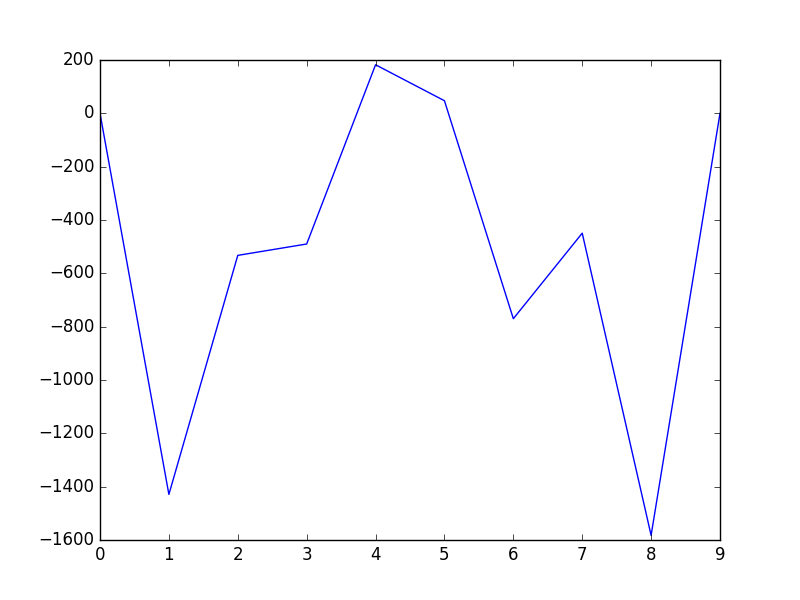
\includegraphics[width=0.4\textwidth]{images/poutre_error.png}
  \caption{}
  \label{beam_error}
\end{figure}



\subsection{Quantification}

We think we can use the FRF method interpolation for a quantification of the damage. For that, we have compared the threshold and the difference between it and the computed error.

We shows in Figure \ref{quant} the computed error, in percent of the threshold. We can see that its evolution is linear against the damage percent.
It could permit to quantify the damage.

\begin{figure}[h!]
  \centering
  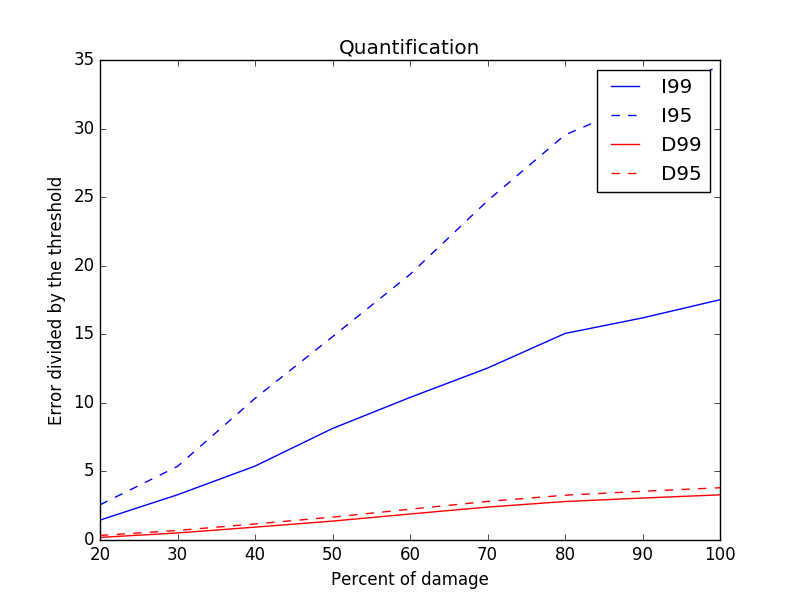
\includegraphics[width=0.4\textwidth]{images/quantification.png}
  \caption{}
  \label{quant}
\end{figure}


\section{Conclusion}

In this paper, we presented the structure health monitoring and a state of the art for this. Then we detailed one of the methods, the FRF interpolation method, and some physical models. Last, we presented our simulation and our results with the implementation of the FRF interpolation method, and analized them.

%nombre de capteurs, fréquences à considérer
We have seen that the FRF interpolation method works, and we proposed a method for eliminate the false positives, and improve its performance. But we have seen that under 10\% of damage, this method doesn't detect damages all the time. To improve the method on that, a study of the considered frequencies could be usefull. Indeed, we have considered all the frequencies under the maximal frequency of the structure here. A selection of the frequencies could permit to detect damages under 10\% extent.

Another way to study is the impact of the number of sensors on the efficiency of the method. Here, we were placed in the ideal case where there is a sensor on each mass. For practice cases, the efficiency of the method with less sensors (for example, one sensor for two masses) should be studied.

%\nocite{*}
\printbibliography

\end{document}
